\chapter{La variazione delle variabili su 24 ore}
\label{app:variazione}

La Figura~\ref{fig:era5-variazione} riporta per tutte le variabili le percentuali della variazione quadratica media su 24 ore discusse nella Sezione~\ref{sec:dati-caratteristiche}.

\begin{figure}[!htb]
    \centering
    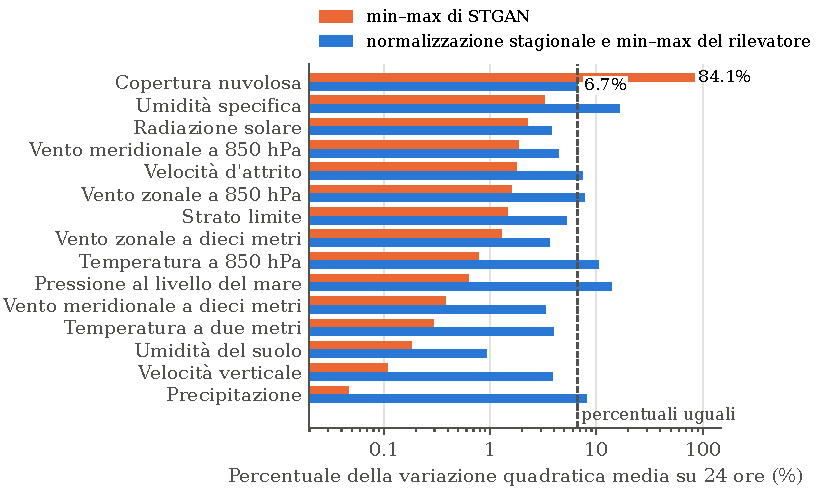
\includegraphics[width=\textwidth]{era5_variazione_24h}
    \caption{Percentuale di ciascuna variabile nella variazione quadratica media su 24 ore, dopo il min--max di STGAN e dopo la normalizzazione stagionale e il min--max del rilevatore, in scala logaritmica; il tratteggio indica un quindicesimo. Anni 1980--1999. Con il solo min--max domina la copertura nuvolosa.}
    \label{fig:era5-variazione}
\end{figure}
